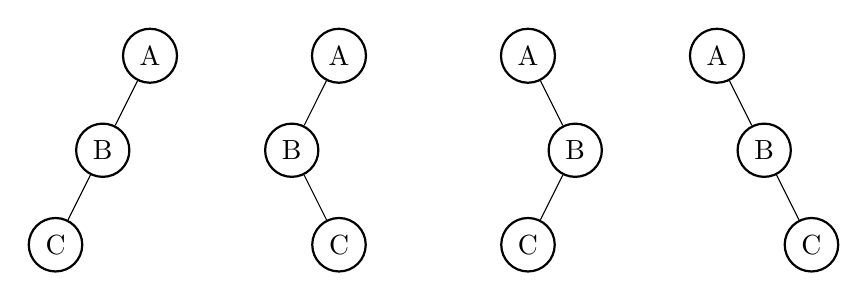
\begin{tikzpicture}[scale=0.8]

  \tikzstyle{every node}=[thick,draw]
  \node[circle] at (0,0) {A}
  child { node[circle]{B}
    child { node[circle]{C}}
    child[fill=none] {edge from parent[draw=none]}  
  }
  child[fill=none] {edge from parent[draw=none]};

  \node[circle] at (3,0) {A}
  child { node[circle]{B}
    child[fill=none] {edge from parent[draw=none]}  
    child { node[circle]{C}}
  }
  child[fill=none] {edge from parent[draw=none]};


  \node[circle] at (6,0) {A}
  child[fill=none] {edge from parent[draw=none]}
  child { node[circle]{B}
    child { node[circle]{C}}
    child[fill=none] {edge from parent[draw=none]}  
  };

  \node[circle] at (9,0) {A}
  child[fill=none] {edge from parent[draw=none]}
  child { node[circle]{B}
    child[fill=none] {edge from parent[draw=none]}
    child { node[circle]{C}}
  };

\end{tikzpicture}
